\chapter{Fundamentação Teórica}
	\label{ch:fundamentacao}
Nesta sessão serão descritos alguns dos conceitos essenciais para a compreensão do trabalho. Inicialmente sera explicado como funciona a organização Baja SAE e as provas a quais os carros são submetidos, além de um breve resumo da história da equipe Velociraptor. Também são descritos alguns detalhes técnicos de quais sensores são/devem ser aplicados no percurso do trabalho alem de informações sobre os microprocessadores estudados para servir como base do \textit{SCOB} vão ser discutidas. Por último é feito uma análise de práticas de engenharia de \textit{software} que podem ajudar na construção do sistema que será proposto.

\section{Baja SAE}
A categoria Baja, organizado pela SAE (\textit{Society of Automotive Engineers}), é uma categoria de \textit{motorsport} feita para estudantes de engenharia aprofundarem seu conhecimento na área com um projeto real, no qual toda a construção do veículo deve ser realizada, bem como sua documentação e busca por patrocinadores para viabilização do projeto. Os carros a serem montados devem, por regulamento, \cite{regulamentobajasae} serem feitos de uma estrutura tubular de aço, fibra de vidro, carbono ou kevlar \cite{projetoMiniBaja2006}, com quatro ou mais rodas e motor padrão de 10HP. Também segundo o regulamento o carro deve suportar uma pessoa de até um metro e noventa de altura e 113,4 quilogramas de peso. Todo o sistema de suspensão, freio, transmissão e chassi é projetado e executado pela equipe participante.  

As provas realizadas pelos veículos em um torneio , segundo \cite{bajasae} são:
\begin{itemize}
	\item Segurança;
	\item Motor;
	\item Conforto;
	\item Frenagem;
	\item Suspensão;
	\item Capacidade de tração;
	\item Dirigibilidade; e
	\item Enduro.
\end{itemize}

Além destas provas a equipe também deve realizar uma apresentação com o projeto completo do veículo, contando pontos para o torneio. A equipe que obtiver a maior quantidade de pontos nas provas citadas acima ganha o torneio.

\section{Sensores}
\label{sec:sensores}
Os sensores, junto com atuadores, são os métodos em que circuitos elétricos conseguem se comunicar com o mundo físico realizando algumas tarefas como fazer uma medida de alguma grandeza. Em \citeonline{Fraden2016} o sensor é definido como "um dispositivo que recebe um estimulo e responde com um sinal elétrico". Existem diversos tipos de sensores e tipos de variações específicas para cada área de uso, sensores de posição como os potenciômetros, sensores de velocidade angular como tacômetros com rotores dentados, sensores de proximidade com uso de sensores óticos e assim por diante \cite{kilian2001modern}. 

Os sensores presentes em um veículo se dividem em duas categorias \cite{vehicleDataAcquisition2014} - aqueles que são feitos para o conforto do passageiro e aqueles feitos para garantir o funcionamento devido da parte dinâmica do veículo. O primeiro é importante para a lista de opcionais do carro consequentemente agradar ao consumidor comum. O segundo é critico ao engenheiro em alto nível, sem impacto imediato para o publico em geral.

Um bom exemplo de como o sensoriamento pode ajudar no desempenho de uma equipe de automobilismo em tempo real é dado por \citeonline{projetoMiniBaja2006}. Quando superaquecido, o motor fica fora do seu regime ideal de trabalho, causando um maior desgaste dos componentes internos e por consequência uma perda de rendimento, o autor continua e comenta que quando o motor esta numa temperatura muito abaixo da ideal, o rendimento também sofre alteração, porque o consumo de combustível aumenta e o torque é menor em relação a um motor ajustado. Para manter o processo dentro de uma faixa desejada, sensores de temperatura do óleo devem ser instalados, com eles é possível manter um histórico da faixa de funcionamento do motor e além de manter o piloto constantemente atualizado da temperatura do motor do seu veículo, o que permite que o piloto tenha mais liberdade em forçar o carro para melhorar o tempo de volta ou dirigir mais cautelosamente, a fim de evitar desgaste excessivo nas peças e melhor consumo de gasolina, fatores que devem ser levados em consideração em uma prova de automobilismo. 

O projeto do veículo \textit{off-road} do grupo Velociraptor já conta atualmente com alguns sensores. A Figura \ref{fig:sensoresBaja} mostra o esquema do sistema elétrico usado atualmente no veículo. Os espaços em azul são sensores utilizados na competição, os espaços em vermelho são sensores usados para testes. 

\begin{figure}[!htb]
	\centering
		\caption{Diagrama do sistema elétrico usados atualmente no baja.}
		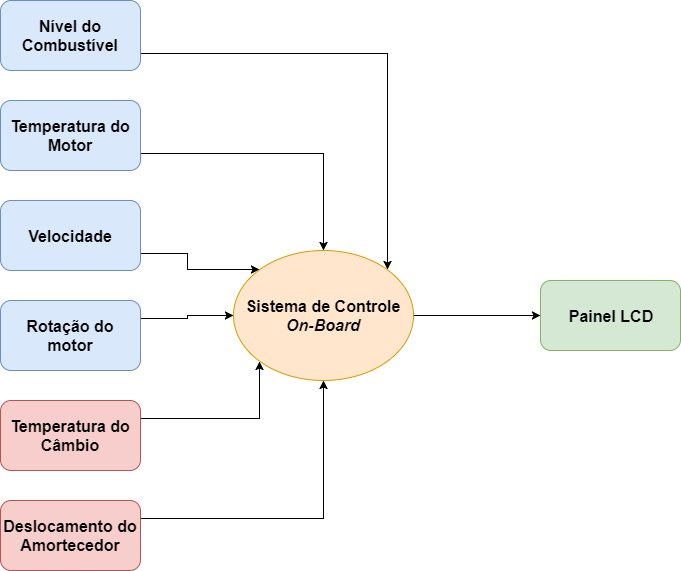
\includegraphics[scale=0.35]{sensoresBaja} 
		\caption*{Fonte: Autor.}
		\label{fig:sensoresBaja}
\end{figure} 

As subseções a seguir explicam o funcionamento destes sensores.

\subsection{Temperatura do motor}

O motor deve operar em uma temperatura ideal abaixo de 110$^\circ$C para desempenhar bem o seu papel. Se sobreaquecidas, as peças do conjunto começam a operar de forma incorreta e isto pode ocasionar rompimento da junta de vedação da galeria de óleo, diminuição da espessura do óleo e em casos de exposição prolongada a sobreaquecimento, travamento do pistão dentro da câmara do motor. Para evitar casos como estes citados acima é importante ter a informação sobre a temperatura do motor, com a informação o piloto pode forçar menos o motor na prova para manter a temperatura estável ou o carro pode ser parado para uma manutenção de emergência.

Para realizar a aquisição desta grandeza é utilizado um sensor termistor de coeficiente negativo de temperatura (conhecido como NTC). Este sensor é normalmente encontrado em lojas de eletrônica da forma demonstrada na Figura \ref{fig:sensorTemperaturantc}, porém, o utilizado no projeto baja Velociraptor é preparado para o ambiente automotivo com um corpo metálico para proteção contra ruídos e melhor posicionamento do sensor. A Figura \ref{fig:sensorTemperaturaautomotivo} é um desenho que demonstra qual é a composição deste sensor. O sensor vai acoplado ao cárter do motor, submerso em óleo. O sensor emite um sinal analógico proporcional a temperatura que ele é exposto, a resistência dele diminuí de acordo com o aumento de temperatura e aumenta com temperaturas mais baixas \cite{Fraden2016}.  

\begin{figure}[ht]
	\center
	\caption{Sensor termistor NTC e um exemplo do sensor específico para automóveis.}
	\subfigure[Fonte:Google Imagens][Sensor termistor NTC. Fonte:Google Imagens]{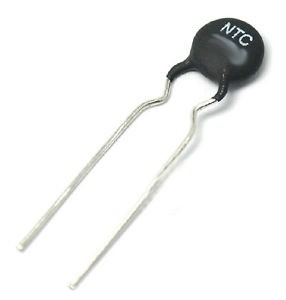
\includegraphics[width=5cm]{sensorTemperatura}\label{fig:sensorTemperaturantc}}
	\qquad
	\subfigure[Fonte:Franscisco Albero S.A.U.][Variante do termistor para aplicação automotiva. Fonte:Franscisco Albero S.A.U. modificado pelo autor]{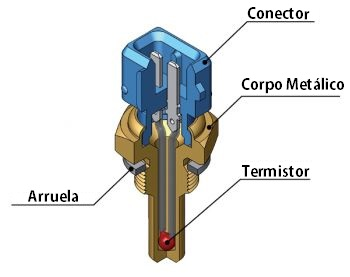
\includegraphics[width=5cm]{sensorTemperaturaautomotivo}\label{fig:sensorTemperaturaautomotivo}}
	\label{fig:sensorTemperatura}
\end{figure}

\subsection{Frequência de rotação do motor}

A revolução/rotação por minuto (RPM) é uma grandeza que indica quantas rotações por minuto um certo objeto realiza, sendo em torno de si mesmo ou em torno de um outro objeto. No contexto do automobilismo, a RPM é a quantidade de vezes em que um motor realiza um giro completo, movendo o virabrequim que esta conectado a uma transmissão. Esta transmissão esta conectada a um eixo e consequentemente o eixo está conectado a roda. Esta é uma ideia básica de como funciona o sistema de conversão de um fenômeno químico (combustão do motor) em força física e o que o RPM trata neste meio.

Para fazer aquisição desta grandeza, é utilizado uma técnica que envolve a vela. A vela, que pode ser vista na Figura \ref{fig:vela}, está presente em todos os carros movidos a motores de combustão, sua função é causar a centelha que começa o processo de explosão do combustível misturado com ar na câmara interna do motor.       

\begin{figure}[!htb]
	\centering
		\caption{Vela automotiva.}
		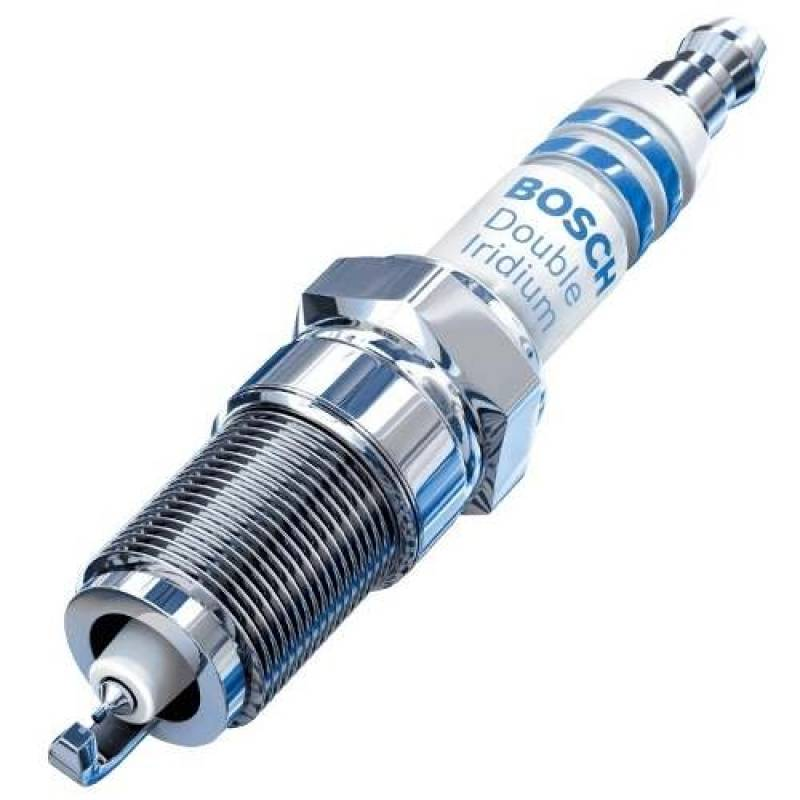
\includegraphics[scale=0.15]{velaAutomotiva} 
		\caption*{Fonte: Google Imagens.}
		\label{fig:vela}
\end{figure} 

A vela produz uma centelha a cada ciclo de explosão da gasolina e esta centelha é produzida a partir de uma carga de energia de 15V. A carga de energia é capturada por uma bobina em volta do fio elétrico da vela e conectada a uma entrada digital do microprocessador. Quando ocorrer a centelha é executada uma interrupção no programa do microprocessador e incrementado um valor em uma variável reservada para o RPM. Esta variável ainda deve ser tratada antes de ser passada para o painel pois a centelha da vela é ativada uma vez a cada ciclo do motor, porém dentro de um ciclo completo (admissão, compressão, explosão e exaustão) é realizado dois giros do virabrequim, ou seja, duas RPM. Depois de ter o valor multiplicado por dois, o valor é demostrado no painel. 

\subsection{Velocidade do veículo}

A velocidade do veículo é a grandeza que indica a quão rápido um veículo se move de um ponto A para um ponto B. Para aquisição desta grandeza é utilizado um sensor MTE 73020 que pode ser visto na Figura \ref{fig:sensorVelocidade}. Este sensor vai acoplado perto do eixo do veículo e captura a rotação do mesmo graças ao efeito Hall, esta rotação é transformada em uma onda quadrática com frequência proporcional a velocidade do veículo \cite{MTEsensorVelocidade} e que deve ser tratada de acordo com a sua aplicação. Este sensor é utilizado em carros da marca GM.  

\begin{figure}[!htb]
	\centering
		\caption{Sensor de velocidade MTE 73020.}
		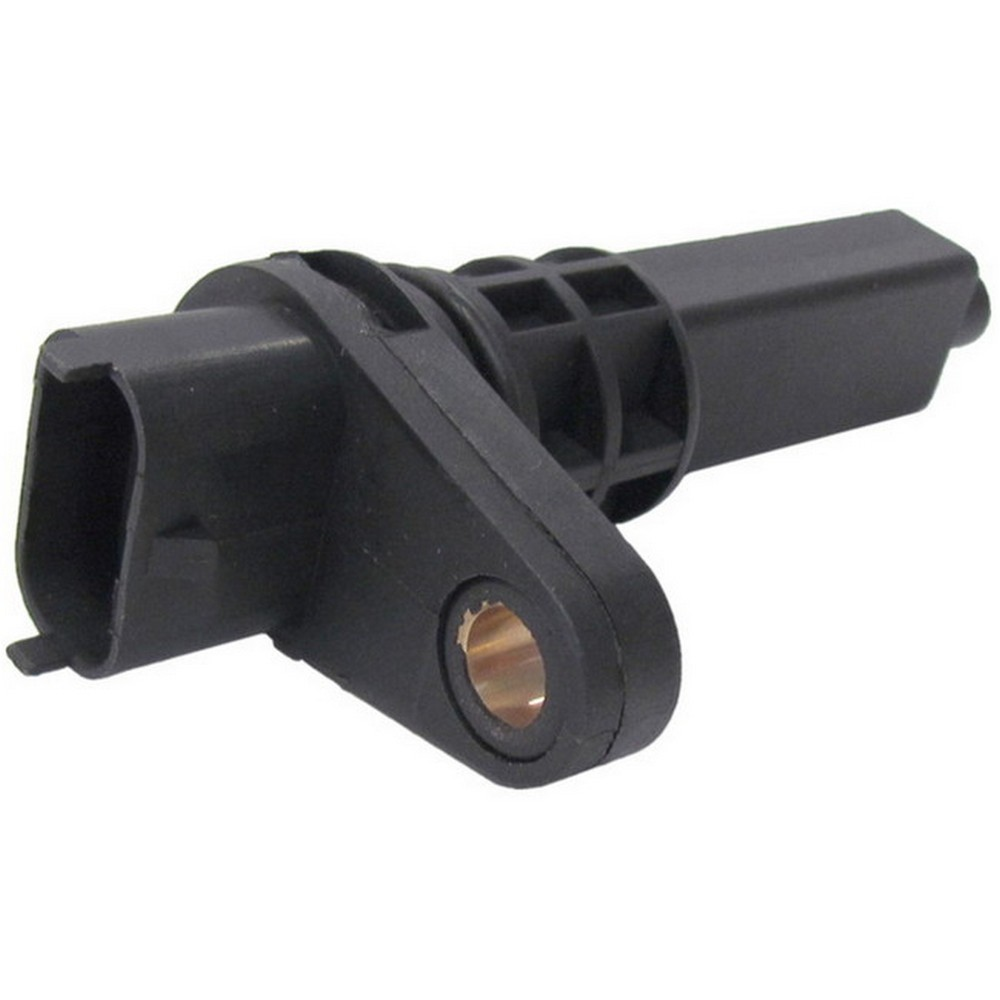
\includegraphics[scale=0.25]{sensorVelocidade} 
		\caption*{Fonte: MTE-THOMSON.}
		\label{fig:sensorVelocidade}
\end{figure} 

No baja Velociraptor o sensor esta acoplado ao eixo traseiro, próximo ao motor, e captura a rotação do freio traseiro que está conectado ao eixo, como pode ser visto na Figura \ref{fig:sensorVelocidadeEx}. Toda vez que um dente do freio passa próximo ao sensor o mesmo emite um sinal quadrático que está conectado a entrada digital do microprocessador no SCOB. A frequência recebida pelo SCOB é tratada, levando em consideração o tamanho da roda e número de dentes no freio, resultando na fórmula matemática a seguir:

\begin{figure}[!htb]
	\centering
		\caption{Sensor de velocidade conectado próximo ao freio traseiro.}
		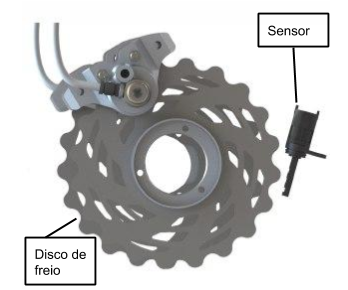
\includegraphics[scale=0.5]{sensorVelocidadeEx} 
		\caption*{Fonte: UDESC Baja Velociraptor.}
		\label{fig:sensorVelocidadeEx}
\end{figure} 

	$$V = \frac{S_{vel}}{N_{freio}} \times 2 \pi r  \times \frac{3.6km}{h}$$  

Aonde $V$ é a velocidade final mostrada no painel, $S_{vel}$ é o número de vezes que o sensor produziu um sinal quadrático, $N_{freio}$ é a quantidade de dentes presente no freio customizado do baja Velociraptor, $2 \pi r$ é fórmula da área da roda e $\frac{3.6km}{h}$ transforma o resultado de metros por segundo para quilômetros por hora.

\subsection{Nível do combustível}
\label{subsec:combustivel}

O combustível é utilizado para causar a explosão controlada dentro do motor de combustão. Medir a quantidade ainda disponível no tanque de gasolina dele é essencial para que possam ser tomadas decisões como manter o veículo na pista ou chamar o veículo para os boxes. A técnica mais comum utilizada para tirar esta grandeza é a boia, como pode ser visto em alguns trabalhos analisados (\cite{Nunes2016} e \cite{projetoMiniBaja2006}) mas esta técnica não pode mais ser aplicada nas competições devido a novas regras de competição que não permitem uso de fios dentro de motores ou tanques de combustível \cite{regulamentobajasae}. 

Para se adequar a estes novos regulamentos, foi utilizada uma nova técnica de medida da grandeza. Esta técnica consistem em utilizar uma boia dentro do tanque de gasolina com um imã e 5 sensores de efeito Hall US1881 fixados pelo lado de fora do tanque. Os sensores de efeito Hall tem seu valor de saída alterado quando a boia presente dentro do tanque passa por ele, desta forma é possível medir a quantidade de gasolina dentro do tanque sem que a necessidade de fios na parte interna do mesmo. A sinal de saída desses sensores é digital, mas para melhor manutenção dos chicotes elétricos este sinal é convertido para um sinal analógico, no qual a frequência recebida pelo microcontrolador é proporcional a quantidade de gasolina presente no tanque. A Figura \ref{fig:sensorTanque} mostra como é montado o \textit{shield} com os sensores de efeito Hall enfileirados.  

\begin{figure}[!htb]
	\centering
		\caption{\textit{Shield} criado para sensores de efeito Hall US1881.}
		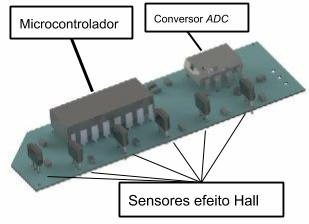
\includegraphics[scale=0.7]{sensorTanque} 
		\caption*{Fonte: UDESC Baja Velociraptor.}
		\label{fig:sensorTanque}
\end{figure} 


\subsection{Temperatura do câmbio CVT}

O motor a combustão de um veículo gera torque e potência, porém esta entrega é linear e pode ser ineficaz dependendo do terreno em que o veículo se encontra. Para contornar esta situação e ter o torque sempre desejado, é adicionada uma transmissão ao veículo. A transmissão converte a saída de torque e potência com o objetivo de manter o motor o mais próximo possível da hipérbole de tração ideal \cite{Naunheimer2011}. 

O tipo de transmissão escolhida para o baja Velociraptor foi uma caixa de câmbio CVT (\textit{Continuosly Variable Transmission}). Para a equipe, a informação da temperatura da transmissão é importante para o projeto do veículo pois o câmbio CVT possui componentes sensíveis como a correia utilizada no sistema. Na Figura \ref{fig:cvt} é possível visualizar um exemplo de câmbio CVT, a correia é o objeto pintado de vermelho e o rompimento da mesma por fatores como desgaste excessivo causaria falha total do sistema. 

\begin{figure}[!htb]
	\centering
		\caption{Câmbio CVT.}
		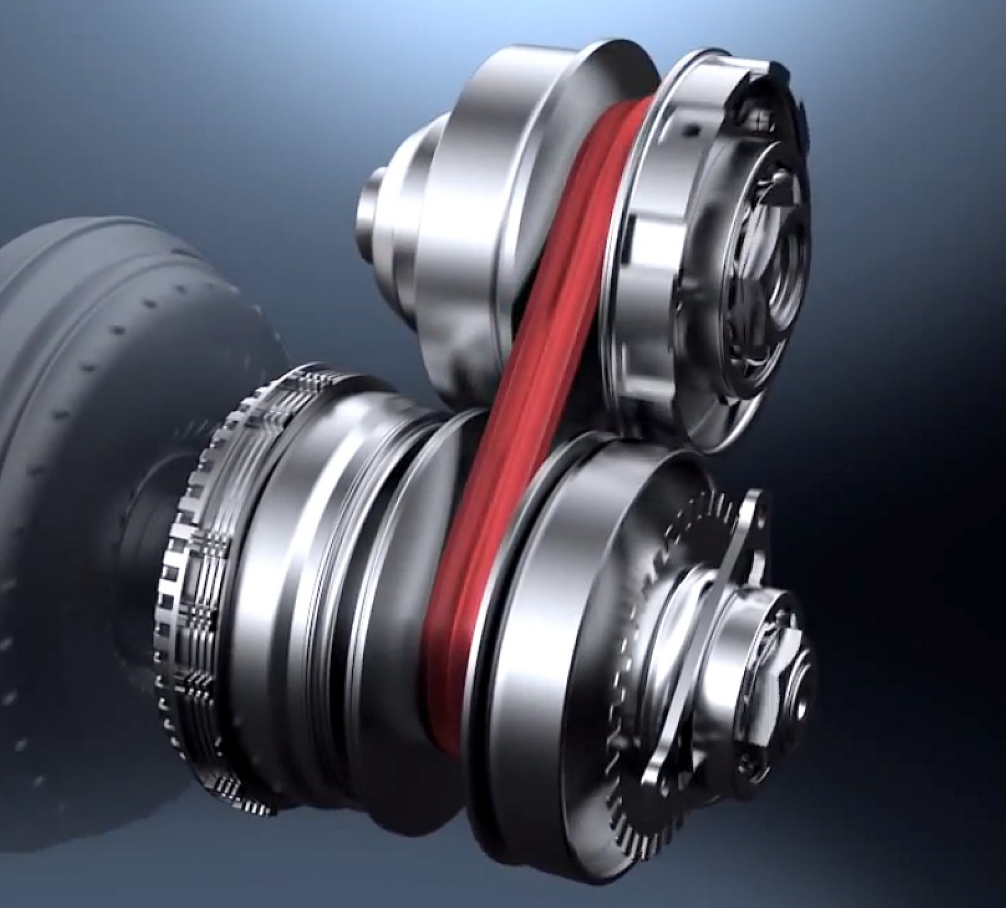
\includegraphics[scale=0.2]{cvt} 
		\caption*{Fonte: Google Imagens.}
		\label{fig:cvt}
\end{figure} 

Para obter essas informações do câmbio foi utilizado um sensor MLX90614 (Figura \ref{fig:sensorCvtimg}). Este sensor, da categoria termopilha, opera utilizando o mesmo princípio de um sensor termopar. Um termopar simples é um dispositivo de baixa sensibilidade que responde a mudanças da casa de 1$^\circ$C com uma mudança de dezenas de $\mu V$, um sensor de termopilha é uma cadeia de termopares conectados, tipicamente 50 a 100 junções, para obter um sinal de 50 a 100 vezes mais forte. O sensor opera com uma membrana com uma capacidade térmica baixa devido a seu tamanho, e esta membrana varia de temperatura de acordo com a radiação térmica para que desta forma a temperatura seja calculada gerando uma voltagem correspondente \cite{Fraden2016}. A Figura \ref{fig:sensorCvtfunc} exemplifica este processo descrito. A saída deste sensor é analógica e vai conectada a entrada analógica do microcontrolador.       

\begin{figure}[!htb]
	\center
	\caption{Sensor MLX90614 e seu funcionamento.}
	\subfigure[Fonte:Google Imagens][Sensor MLX90614. Fonte:Google Imagens]{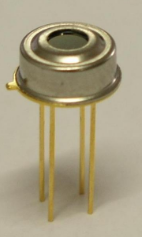
\includegraphics[width=5cm]{sensorCvt}\label{fig:sensorCvtimg}}
	\qquad
	\subfigure[Fonte:\cite{Fraden2016}][Exemplo do funcionamento. Fonte:\cite{Fraden2016}]{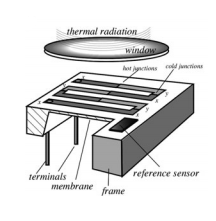
\includegraphics[width=5cm]{sensorCvtfunc}\label{fig:sensorCvtfunc}}
	\label{fig:sensorCvt}
\end{figure}

\subsection{Deslocamento do amortecedor}

O amortecedor, que está contido no conjunto da suspensão, tem o papel de controlar o carro de forma a manter as rodas do veículo em constante contato com o solo, trazendo melhor desempenho para o mesmo. Este sensor de deslocamento de amortecedor é utilizado em bancada para testes e para realização da aquisição da grandeza, neste caso a distância de deslocamento, foi criado um instrumento semelhante a um amortecedor em cano PVC e este instrumento fica acoplado ao lado do amortecedor. Quando o amortecedor sofre tensão o esforço também é transmitido para o instrumento e nele é realizada a aquisição da grandeza. Estes dados adquiridos ajudam na tomada de decisão da configuração da suspensão, escolhendo entre uma suspensão mais rígida ou mais suave dependendo do terreno, calibragem dos pneus, etc...     

É utilizado um sensor GP2Y0A21YK0F da SHARP como pode ser visto na Figura \ref{fig:sensorAmortecedor} para fazer a aquisição do deslocamento do amortecedor. Este sensor vai acoplado em uma das pontas do cano, apontado para a outra. A distância efetiva de operação do sensor é de 10cm - 80cm \cite{SHARP} o que é suficiente para o cenário. O sinal resultante da aquisição é analógico e proporcional a distância do sensor em relação ao objeto em que ele está apontado. 


\begin{figure}[!htb]
	\centering
		\caption{Sensor de deslocamento do amortecedor SHARP GP2Y0A21YK0F.}
		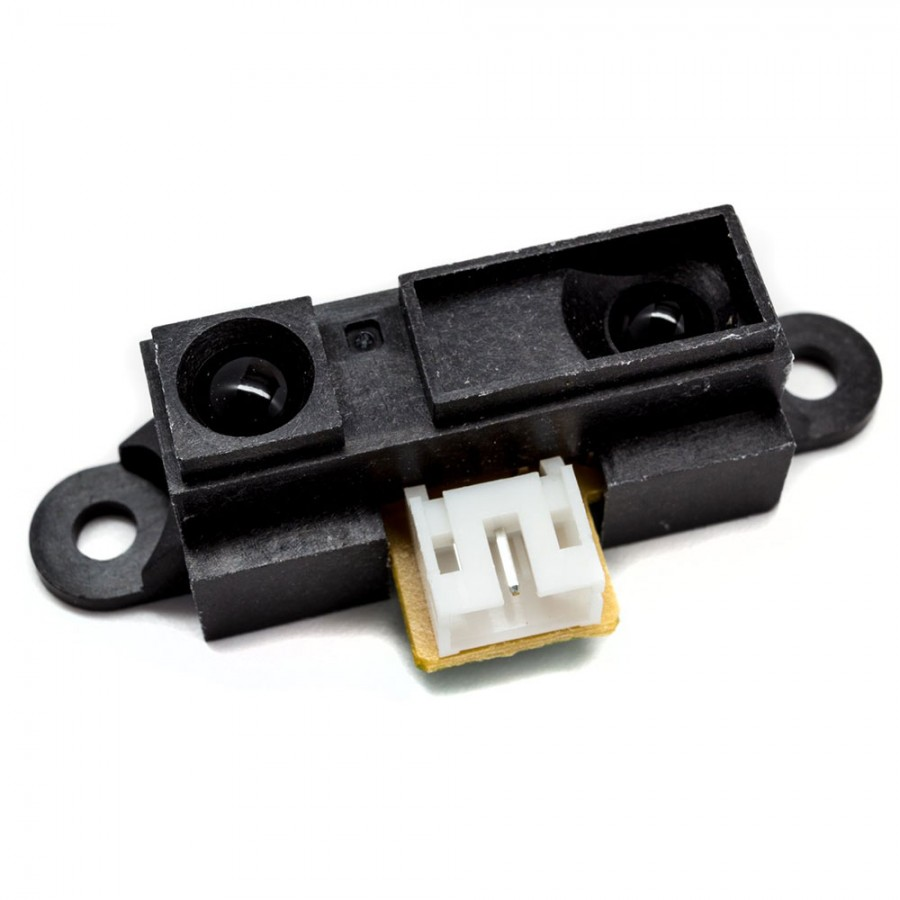
\includegraphics[scale=0.15]{sensorAmortecedor} 
		\caption*{Fonte: SHARP.}
		\label{fig:sensorAmortecedor}
\end{figure} 


\section{Microcontroladores}
\label{sec:microcontroladores}

Os microcontroladores são os dispositivos de maior importância dentro de um sistema embarcado, sendo considerados o coração de um projeto que envolva soluções remotas \cite{aSurveyTo2010}. O microcontrolador possui várias funções integradas dentro de um único chip e com baixo consumo de energia. Dentro dele é possível encontrar uma unidade de processamento, uma quantidade fixa de memória RAM, memória ROM, pinagem para operações gerais de entrada e saída, entradas/saídas para protocolos seriais como \textit{I$^2$C} além de um \textit{timer} \cite{mazidi2008pic}. A Figura \ref{fig:arquiteturaAtmega} é um exemplo a arquitetura de um microcontrolador usado em diversas placas de desenvolvimento, o ATmega328/ATmega328p. Ele utiliza arquitetura Harvard, ou seja, o acesso a memória de dados é separado da memória de programa.        


\begin{figure}[!htb]
	\centering
		\caption{Diagrama de blocos do microcontrolador ATmega328/ATmega328p.}
		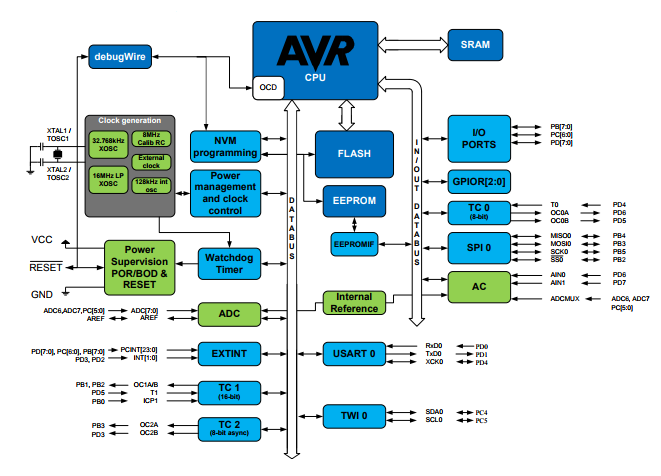
\includegraphics[scale=0.7]{arquiteturaAtmega} 
		\caption*{Fonte: Atmel.}
		\label{fig:arquiteturaAtmega}
\end{figure} 

Em \citeonline{aSurveyTo2010} e em \citeonline{mazidi2008pic} são citados alguns fatores que são levados em conta na escolha do microcontrolador, porém tais critérios podem ser revistos e redimensionados para a aplicação no baja Velociraptor. Os critérios de maior relevância então são:

\begin{itemize}
	\item Baixo consumo de energia;
	\item Quantidade de RAM e ROM suficiente para a rotina desejada;
	\item Facilidade de desenvolvimento;
	\item Quantidade suficiente de entradas/saídas para periféricos; 
	\item Programável em C; e
	\item Custo.
\end{itemize}   

A equipe Velociraptor atualmente já trabalha com um microcontrolador da Atmel, o ATmega328 em uma placa de desenvolvimento Arduino Nano V3. Este microcontrolador supre todos os critérios citados acima para o cenário atual, com os sensores citados na seção \ref{sec:sensores}, porém com a criação de um novo \textit{software} para tratamento de dados e em conjunto com os objetivos futuros da equipe de atualizações nas tecnologia utilizadas, o uso deste microcontrolador deve ser revisado para ser mantido ou descartado. Outro fator discutido com a equipe é o uso de microcontroladores que são suportados por placas de desenvolvimento, revisadas na seção \ref{sec:placasdedesenvolvimento}. As placas de desenvolvimento facilitariam a criação do SCOB, e servem para o escopo deste projeto já que são placas desenvolvidas para um ambiente de prototipagem. 

a Tabela \ref{tab:microcontroladores} faz uma comparação entre microcontroladores encontrados em placas de desenvolvimento no mercado das marcas Intel\footnote{\href{https://www.intel.com/content/dam/www/public/us/en/documents/datasheets/quark-c1000-datasheet.pdf}{Quark SE Microcontroller C1000 Datasheet}}, Atmel\footnote{\href{http://www.atmel.com/Images/Atmel-7766-8-bit-AVR-ATmega16U4-32U4_Datasheet.pdf}{ATmega16U4/ATmega32U4 Datasheet}}\footnote{\href{http://www.atmel.com/Images/Atmel-42735-8-bit-AVR-Microcontroller-ATmega328-328P_Datasheet.pdf}{ATmega328/P Datasheet}}\footnote{\href{http://www.atmel.com/Images/Atmel-2549-8-bit-AVR-Microcontroller-ATmega640-1280-1281-2560-2561_datasheet.pdf}{Atmel ATmega640/V-1280/V-1281/V-2561/V Datasheet}}\footnote{\href{http://www.atmel.com/Images/Atmel-11057-32-bit-Cortex-M3-Microcontroller-SAM3X-SAM3A_Datasheet.pdf}{SAM3X / SAM3A Series Datasheet}} e NXP\footnote{\href{https://www.nxp.com/docs/en/data-sheet/KL25P80M48SF0.pdf}{NXP Kinetis KL25 Sub-Family Datasheet}} . 
O microcontrolador com maior poder de processamento é o AT91SAM3X8E com velocidade de \textit{clock} 5.25 vezes maior que o microcontrolador com mais lento e 48 vezes mais memória. O microcontrolador da Intel possui uma boa quantidade de memoria RAM, porém sua pinagem é menor que do ATmega328, o microcontrolador de menor desempenho da família Atmel visto neste comparativo. 
\begin{table}[!htb]
	\centering
	\caption{Comparação de microcontroladores }
	\label{tab:microcontroladores}
	\begin{tabular}{|l|l|l|l|l|l|}
		\hline
		\rowcolor[HTML]{9B9B9B} 
		\textbf{Modelo}  & \textbf{Fabricante} & \textbf{Clock} & \textbf{I/O Digital} & \textbf{I/O Analógica} & \textbf{RAM} \\ \hline
		AT91SAM3X8E    & Atmel               & 84 MHz         & 54                   & 14                     & 96 KB SRAM   \\ \hline
		ATmega2560     & Atmel               & 16 MHz          & 54                   & 16                     & 8 KB SRAM    \\ \hline
		ATmega328     & Atmel               & 16 MHz         & 14                   & 8                      & 2 KB SRAM    \\ \hline
		ATmega32u4     & Atmel               & 16 MHz          & 20                   & 12                     & 2.5 KB SRAM  \\ \hline
		MKL25Z128VLK4  & NXP                 & 48 MHz          & 60                   & 6                      & 16 KB SRAM   \\ \hline
		Quark SE C1000 & Intel               & 32 MHz         & 14                   & 6                      & 80 KB SRAM   \\ \hline
		\end{tabular}
	\caption*{Fonte: Autor.}
\end{table}

\subsection{Placas de desenvolvimento} 
\label{sec:placasdedesenvolvimento}

O mercado atual de sistemas embarcados oferece uma opção para melhor produtividade e facilidade de desenvolvimento, a custo da especificidade envolvida nos projetos. As placas de desenvolvimento são componentes criados para suportar um ambiente com uma unidade de processamento, geralmente um microcontrolador, um cristal gerador de \textit{clock} e uma entrada para interfaceamento com o computador (USB ou mini-USB), outros periféricos também podem ser encontrados de fábrica dependendo do modelo, como acelerômetros e giroscópios. 

Estas placas de desenvolvimento possuem diversos microcontroladores, fabricantes, tamanhos, poder de processamento, poder de armazenamento e assim por diante. A Tabela \ref{tab:placasdedesenvolvimento} traz uma comparação entre várias placas de desenvolvimento que utilizam microcontroladores vistos na Tabela \ref{tab:microcontroladores}. A dimensão é dada em milímetro, todas as placas tiveram seus preços verificados no mês de novembro do ano 2017 em um \textit{e-commerce} de componente eletrônicos\footnote{https://www.filipeflop.com/}. A dimensão de altura das placas Arduino são estimativas, visto que oficialmente estes números não são divulgados. 

\begin{table}[!htb]
	\centering
	\caption{Comparação entre placas de desenvolvimento}
	\label{tab:placasdedesenvolvimento}
	\begin{tabular}{|l|l|l|l|l|}
	\hline
	\rowcolor[HTML]{9B9B9B} 
	\textbf{Modelo}      & \textbf{Fabricante} & \textbf{Microcontrolador} & \textbf{Dimensões} & \textbf{Preço} \\ \hline
	FRDM-KL25Z		   & NXP                 & MKL25Z128VLK4             & 80 x 53 x 6        & R\$169,90      \\ \hline
	Genuino 101        & Intel               & Quark SE                  & 70 x 55 x 20       & R\$229,90      \\ \hline
	Uno R3             & Arduino             & ATmega328                 & 68.6 x 53.4 x 25   & R\$44,90       \\ \hline
	Nano V3            & Arduino             & ATmega328                 & 45 x 18 x 7.6      & R\$49,90       \\ \hline
	Mega 2560 R3       & Arduino             & ATmega2560                & 102 × 54 x 25      & R\$74,90       \\ \hline
	Due                & Arduino             & AT91SAM3X8E               & 101.52 x 53.3 x 25 & R\$139,90      \\ \hline
	Leonardo R3        & Arduino             & ATmega32u4                & 68.6 x 53.3 x 25   & R\$59,90       \\ \hline
	\end{tabular}
	\caption*{Fonte: Autor.}
\end{table}

É possível tirar algumas análises desta tabela, por exemplo, o Arduino Nano V3 possui o mesmo poder de processamento de um Arduino Uno R3 porém utiliza uma área aproximadamente 4.5 vezes menor do que o mesmo, custando uma pequena margem a mais. Levando em conta o cenário do projeto, as \textbf{dimensões} de uma placa de desenvolvimento é um fator que também deve ser levado em conta na tomada de decisão, o que não se aplicava a microcontroladores pois estes possuem um tamanho pequeno em comparação com placas de desenvolvimento que possuem alguns componentes extras já citados no início da seção de fábrica. Algumas placas como Genuino 101, Due e FRDM-KL25Z possuem um preço que varia acima da casa dos R\$100, isto pode ser justificado com desempenho superior em relação as demais placas e alguns periféricos extras já inclusos nestas placas, como acelerômetro em ambas FRDM-KL25Z e Genuino 101. Placas com dimensões como o modelo Mega 2560 R3 não são a melhor opção para ser utilizadas no veículo para uso durante a prova visto a impossibilidade de criar um \textit{shield} para proteção da mesma e acoplamento no painel dianteiro do veículo. A Figura \ref{fig:paineldianteiro} da uma demonstração de como está estruturado o painel atualmente com um Arduino Nano V3. Uma mudança de tamanho requisitaria uma revisão do projeto de eletrônica do veículo.

\begin{figure}[!htb]
	\centering
		\caption{Foto do painel dianteiro atual do baja Velociraptor.}
		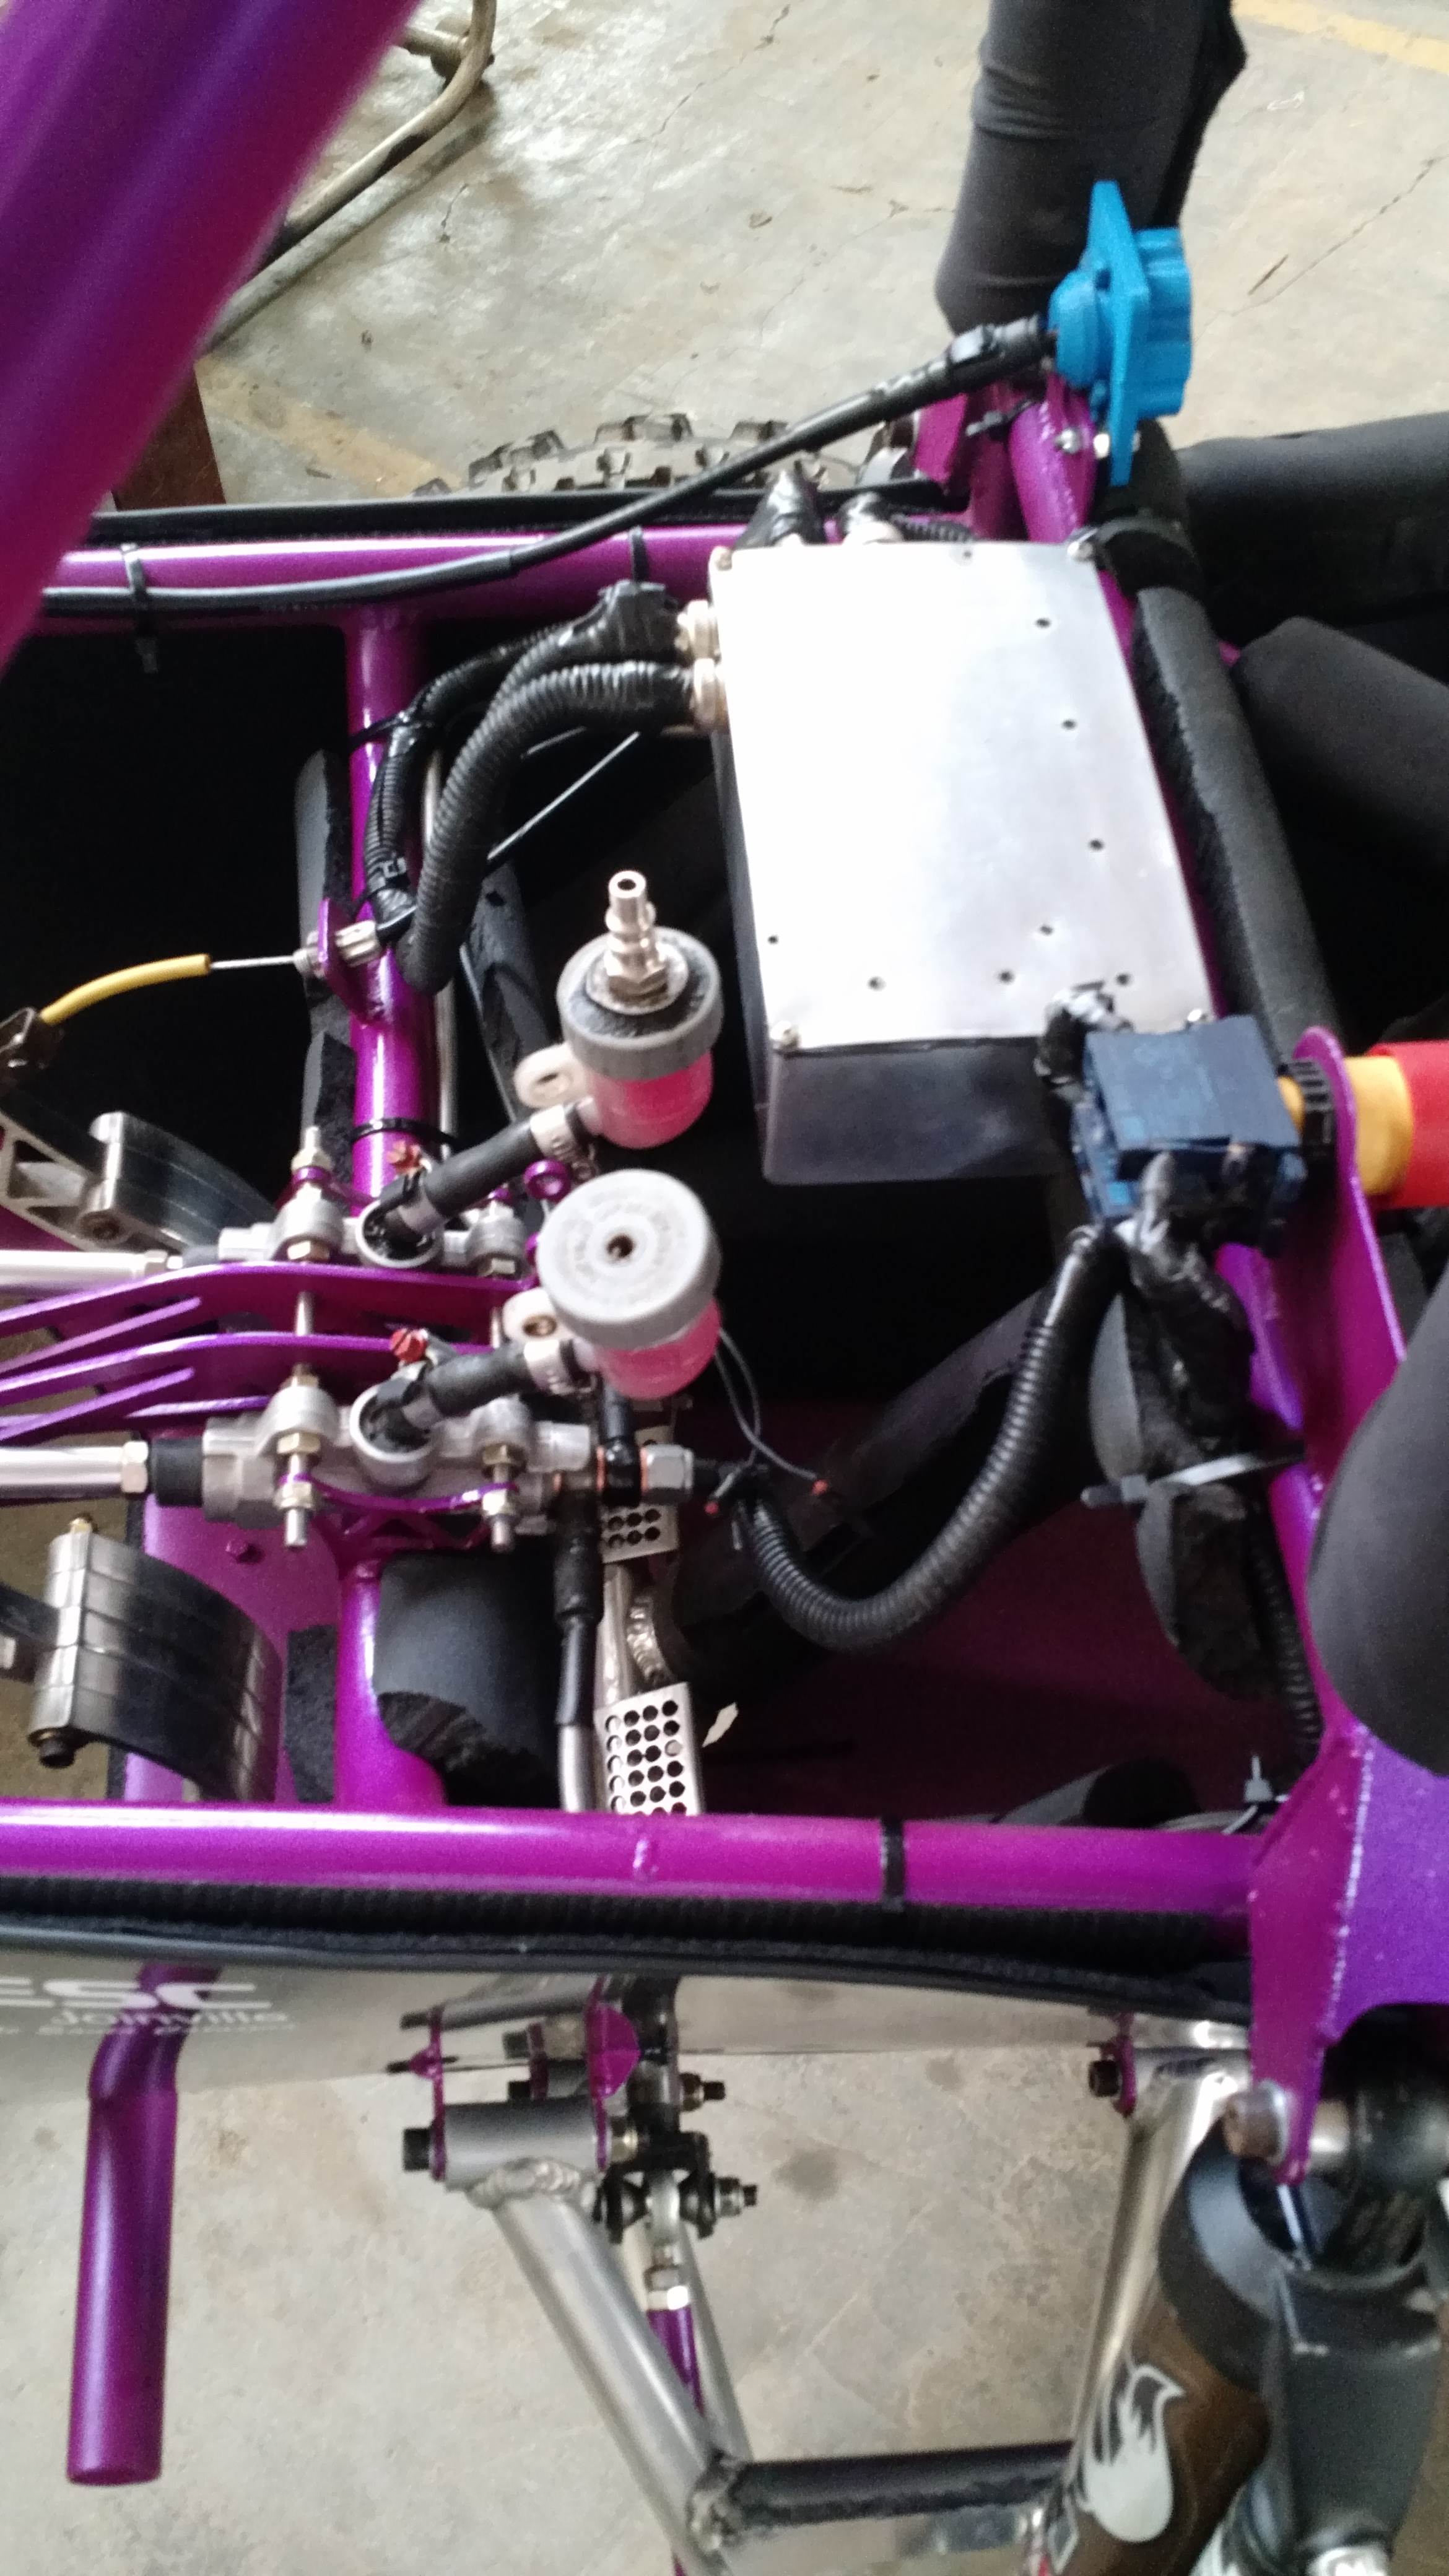
\includegraphics[scale=0.05]{paineldianteiro} 
		\caption*{Fonte: Autor.}
		\label{fig:paineldianteiro}
\end{figure} 
     

Todavia, além das placas de desenvolvimento citadas, \citeonline{designAndImplementation2015} trás uma solução de aquisição de dados para veículos (mais informações do trabalho no capítulo \ref{ch:trabalhos}) com o uso de placas de melhor desempenho, com maior número de periféricos porém ainda em uma escala reduzida. Este tipo de placa é comumente chamado de \textit{Single Board Computer} por serem capazes de rodar um sistema operacional completo, e não apenas um programa como nas placas analisadas na Tabela \ref{tab:placasdedesenvolvimento}. A Tabela \ref{tab:singleboard} tem a comparação de algumas destas \textit{Single Board Computer} na qual as dimensões são dadas em milímetro, todas as placas tiveram seus preços verificados no mês de novembro do ano 2017 em um \textit{e-commerce} de componente eletrônicos\footnote{https://www.filipeflop.com/}.

\begin{table}[!htb]
	\centering
	\caption{Comparação entre \textit{Single Board Computer}}
	\label{tab:singleboard}
	\resizebox{\textwidth}{!}{\begin{tabular}{|l|l|l|l|l|l|l|l|l|}
		\hline
		\rowcolor[HTML]{9B9B9B} 
		\textbf{Modelo} & \textbf{Fabricante} & \textbf{Processador}     & \textbf{Clock} & \textbf{I/O Digital} & \textbf{I/O Analógica} & \textbf{RAM}  & \textbf{Dimensões} & \textbf{Preço} \\ \hline
		3 Model B     & Raspberry Pi        & BCM2837         & 1200 MHz       & 40                   & N/A                    & 1 GB LPDDR2   & 85 x 56 x 17       & R\$299,90      \\ \hline
		Zero W        & Raspberry Pi        & BCM2835         & 1000 MHz       & 40                   & N/A                    & 512 MB LPDDR2 & 65 x 30 x 5        & R\$79,90       \\ \hline
		Green         & BeagleBone          & AM3358 & 1000 MHz       & 65                   & 7                      & 512 MB DDR3   & 86 x 53 x 19       & R\$329,90      \\ \hline
		Black Rev.C   & BeagleBone          & AM3358 & 1000 MHz       & 65                   & 7                      & 512 MB DDR3   & 86 x 53 x 19       & R\$399,90      \\ \hline
	\end{tabular}}
	\caption*{Fonte: Autor.}
\end{table}

Os modelos 3 Model B, Green e Black Rev.C possuem um preço acima da faixa de R\$250 e dificilmente serão escolhidos para o projeto, porém todas as placas comparadas, o modelo Zero W tem a proposta mais atraente. Com memória RAM de 512 MB, velocidade de \textit{clock} de 1000 MHz, dimensões 65 x 30 x 5 milímetros e preço R\$79,90 esta \textit{Single Board Computer} possui poder de processamento e memória acima dos modelos vistos na Tabela \ref{tab:placasdedesenvolvimento} por um preço abaixo da casa de R\$100. A utilização dessas placas ainda trazem vantagens como a possibilidade de rodar um sistema operacional dentro do veículo, o que pode ser explorado para melhor processamento de dados dentro do SCOB, utilização de linguagens interpretadas e utilização de sistemas gerenciadores de bancos de dados para adição de uma camada extra de confiabilidade nos dados entregues pelo sistema. A desvantagem da utilização deste sistema é o custo, que aumenta uma margem pequena (cerca de 1.6 vezes o valor atual da placa de desenvolvimento), o aumento da complexidade do sistema com a adição de um sistema operacional dentro do veículo, o aumento das dimensões da placa de desenvolvimento (de 45 x 18 x 7.6 para 65 x 30 x 5) e a falta de entradas analógicas no modelo Zero W sendo assim necessário o uso de módulos ADC externos. 

\section{Software}
\label{sec:software}

% ------------------------------------------- PARTE DA ANDRESSA, DEIXAR PARA PEGAR ALGUM EXEMPLO DE ESCRITA
\begin{comment}
	\section{Síntese de Som}
	A síntese sonora é uma técnica de geração de som utilizando equipamentos eletrônicos ou softwares, a partir do zero. O objetivo principal não é imitar sons existentes e sim criar sons totalmente novos. Um sintetizador, um instrumento musical eletrônico como a Figura \ref{fig:sintetizador}, tem a capacidade de emitir sons de piano, flauta, violão, mas o foco é criação de novos sons com timbres diferentes. Como um sintetizador, o computador também é um ferramenta a utilizar-se na síntese sonora.

	\begin{figure}[!htb]
	\centering
		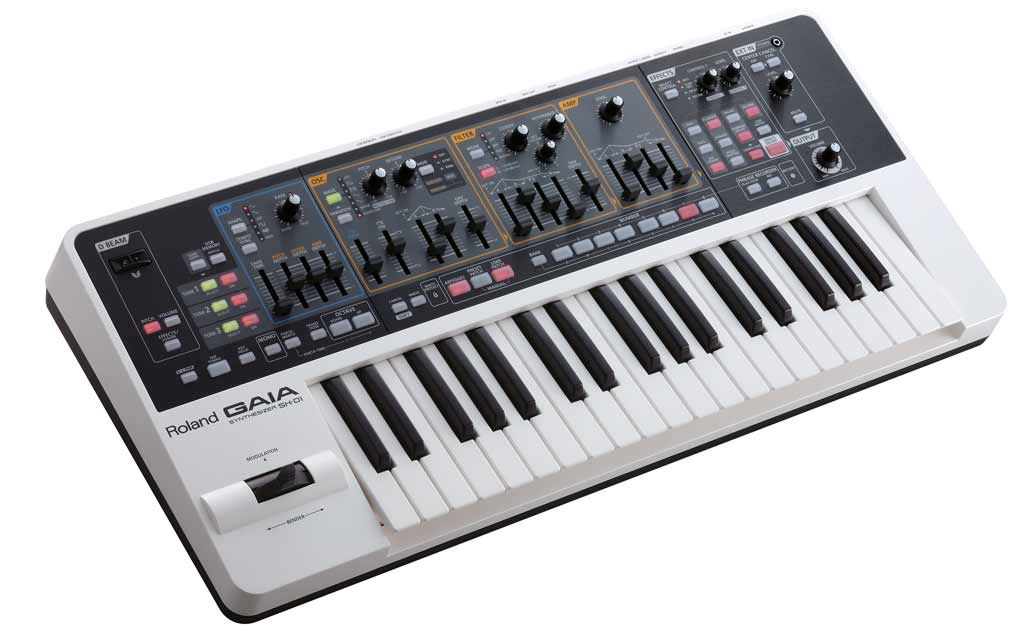
\includegraphics[height=4cm]{sintetizador}
		\caption{Exemplo de sintetizador: Roland Gaia. Fonte: Desconhecido.}
		\label{fig:sintetizador}
	\end{figure}

	Ao escolher técnicas para realizar a síntese há uma vasta gama de técnicas como síntese granular, aditiva, subtrativa entre outras.


	-----------ESCREVER MAIS


	\section{Processo Criativo}
	O processo criativo é importante para o \textit{Live Coding} pela natureza perfomática da arte, fazendo-se necessário abordar sobre composição musical e improvisação.  

	\subsection{Música}
	De acordo com \cite{lacerda1966} a música é a arte dos sons, as principais partes da música são: melodia, ritmo, harmonia.

	\begin{itemize}
		\item Melodia: o conjunto de sons dispostos em ordem sucessiva, é o tema da música, o qual capta a atenção do ouvinte;
		\item Harmonia: o conjunto de sons dispostos de forma simultânea que complementa a melodia;
		\item Ritmo: a ordem e proporção em que estão dispostos os son, definida também como a batida ou marcação do tempo.
	\end{itemize} 

	Esses elementos citados são básicos nas etapas de composição, sendo a melodia a mais importante da composição.

	\subsection{Composição musical}
	A composição musical tem como base o conhecimento do músico em relação a teoria musical e criatividade. É essencial o domínio de alguns fundamentos da teoria musical sobre a melodia, harmonia, ritmo, estilo musical, forma. A criatividade é muito influente na composição, ela está ligada com a ideias, sensibilidade do artista, ambiente onde este artista está inserido e entre outros fatores. A composição descrita aqui está ligada à criação de melodia, harmonia e definição dos instrumentos e não à criação de letra para uma música.  

	O processo da composição acontece em quatro estágios: conscientização da ideia, concepção da forma, escolha do material sonoro definindo os sons e instrumentos presentes, e estruturação estabelecendo repetições e variações sonoras. % \cite{keylist}

	Para um compositor é fundamental conseguir implementar sua criação de uma forma rápida e precisa, não por questões de produtividade, mas sim para poder reagir as suas ideias o mais próximo possível do tempo real \cite{Barbosa1999}. A tecnologia trouxe benefícios para o processo de composição musical. Os ambientes existentes para partitura e composição possibilitam que a melodia ou os arranjos criados possam ser ouvidos rapidamente com \textit{feedback}, logo após a inserção ou modificação da criação. Além de poder usar vários instrumentos diferentes na execução sem requerer a presença de um instrumentista. 	

	----Ao enfocar os processos criativos envolvidos na composição musical, argumentam que “o escasso material que tem sido escrito sobre os processos criativos (em oposição ao produto) no domínio da composição têm sido quase exclusivamente na forma de relatos pessoais [...]”. Por conseguinte, são raros os estudos que investigam os fatores que inspiram os compositores na produção de suas obras


	\subsection{Improvisação musical}	
	A improvisação musical é a arte de compor e registrar ao mesmo tempo, onde o artista expressa em tempo real as suas ideias. É necessário ter domínio do instrumento e de teoria musical, de tal maneira que consiga assimilar rapidamente a ideia e colocá-la em prática. Muitos estilos musicais são baseados na improvisação durante uma performance, Jazz , Blues e música eletrônica são exemplos que possuem essa característica marcante.
\end{comment}